\chapter{The Quantum Hypothesis}

\chapterprecis{Max Planck\footnotemark}

\footnotetext{Indented sections of this chapter describing Planck's 
research are drawn from Robert Resnick, \emph{Basic Concepts in 
Relativity and Early Quantum Theory} (New York: John Wiley and Sons, 
Inc., 1972), 113--116 and 119--123.}

\makeoddhead{myheadings}{\emph{Planck}}{}{\thepage}
\makeevenhead{myheadings}{\thepage}{}{\emph{The Quantum Hypothesis}}

\renewcommand{\theequation}{\arabic{equation}}

The mathematical analysis in Einstein's paper in Chapter VI is connected
to something called ``Planck's quantum hypothesis,'' and Einstein
emphasizes the strength the connection lends to his own argument.
Planck's quantum hypothesis states that microscopic light-emitting
bodies only absorb and emit energy in indivisible units or ``quanta.''
As we shall see in his paper, Einstein adopts this hypothesis and indeed
argues for a radical extension of it. Unfortunately, the work leading up
to this hypothesis involves a great deal of probability theory which we
cannot go into here. But at least the phenomena and the ways of thinking
about them that led to the quantum hypothesis can be sketched.

\section*{A. Black Body Radiation: The Phenomena, First Attempts to
Understand Them, and Planck's \emph{Empirical} Determination of a
Formula to Fit Them.}

Being hot enough will make any solid body glow visibly. The filament in
an incandescent light bulb is not undergoing any chemical reaction: it
is glowing because it is hot. Furthermore, such a glowing body will glow
in a characteristic color and will change color, up or down the spectrum
in order, if it gets hotter or cooler.

For instance, what happens when an iron bar is heated? If its
temperature gets high enough, it starts to glow. Some of the energy
absorbed as heat is given off as light. This emitted light first becomes
visible when it is red-hot. (In fact at lower temperatures a body
``glows'' in the infra-red range, that is, at frequencies too low for
human eyes to see. This is what makes infrared photography possible.) As
the temperature rises the bar changes to other colors, up through the
spectrum, and eventually becomes blue-hot.

Why does it have distinct colors along the way? If the frequencies at
which it can emit light were all equally entitled to an equal share of
the energy, like the piano strings or the air molecules, we'd expect
that the blend of colors given off by the bar would always be the same
and that only the intensity of its glow would increase with increasing
temperature. But, instead, as we heat the bar, it goes through a phase
of intense red, a later phase of intense yellow, etc. For some reason,
at a certain range of temperatures, the bulk of the light-energy is
emitted at the red frequency, but at a higher temperature range yellow
is preferred.

Well before 1900, it was known that electromagnetic waves were absorbed
and emitted by bodies. These waves could be in the form of infrared
radiation (also known as thermal radiation or heat), visible light,
ultraviolet light, or x-rays. Anything that is at a temperature above
absolute zero will emit some kind of light in the infrared.

Nothing can emit for very long unless it is also absorbing light at some
frequency. In general, the more the body absorbs, the more it will emit.
Once a body absorbs light, assuming the body is dense enough, the energy
of the light will come to some kind of equilibrium within the body and
the emitted light will be in a range of frequencies, with a peak at some
frequency that depends on the temperature and, to some extent, on the
make-up of the body. The dependence on the make-up of the body gets less
and less as the body becomes more uniformly dense (so that equilibrium
of frequencies is achieved and conduction and convection do not carry
off some of the heat) and blacker (so that more and more light is
absorbed in order to be emitted).

\begin{quotation}
The radiation emitted by a body as a result of its temperature is called
\emph{thermal radiation}. All bodies emit such radiation to their
surroundings and absorb such radiation from it. If a body is at first
hotter than the surroundings it will cool off because its rate of
emitting energy exceeds its rate of absorbing energy. When \emph{thermal
equilibrium} is reached, the rates of emission and absorption are equal.

Matter in a condensed state (i.e., solid or liquid) emits a continuous
spectrum of radiation. The details of the spectrum depend strongly on
the temperature. At ordinary temperatures most bodies are visible to us
not by their emitted light but by the light they reflect. If no light
shines on them we cannot see them. At very high temperatures, however,
bodies are self-luminous. We can see them glow in a darkened room (hot
coals, e.g.). But even at temperatures as high as several thousand
degrees Kelvin, well over 90\% of the emitted thermal radiation is
invisible to us, being in the infrared part of the electromagnetic
spectrum. Self-luminous bodies are quite hot, therefore.

If we were to steadily raise the temperature of a hot body, we would
observe two principal effects: (1) the higher the temperature, the more
the thermal radiation emitted---at first the body appears dim, then it
glows intensely; and (2) the higher the temperature, the higher the
frequency of that part of the spectrum radiating most intensely-\/-the
predominant color of the hot body shifts from ``red heat'' to ``white
heat'' to ``blue heat.'' Since the quality of its spectrum depends on
the temperature, we can estimate the temperature of a hot body, such as
a star or a glowing chunk of steel, by analyzing the radiation it emits.
There is a continuous spectrum of radiation emitted, the eye seeing
chiefly the color corresponding to the most intense emission in the
visible region.

The detailed form of the spectrum of the thermal radiation emitted by a
hot body at a given temperature depends somewhat upon the composition of
the body. There is one class of hot bodies, however, called \emph{black
bodies}, which emit thermal radiation with the same spectrum at a given
temperature, regardless of the details of their composition. Such bodies
have surfaces that absorb all the thermal radiation incident upon them
and, because they do not reflect light, appear black. An object coated
with a diffuse layer of black pigment, such as lamp black or bismuth
black, is (nearly) a black body. A cavity in a body, open to the outside
by a small hole, is also a black body, as we shall soon explain. A
theoretical understanding of black body, or cavity, radiation was a
major goal of physicists before the turn of the {[}twentieth{]} century.

Consider first the experimental observations. The spectral distribution
of black-body radiation is described by a quantity
$\Re_T(\nu)$ called the \emph{spectral radiancy}, which
is defined so that the quantity $\Re_T(\nu)\,d\nu$ is the
{[}time{]} rate at which energy is radiated per unit area of a surface
at absolute temperature \emph{T} for frequencies in the interval
$\nu$ to $\nu\! +\! d\nu$. In Fig. 1, we show the experimentally
observed dependence
%
\begin{figure}[h]
  \begin{center}
  \captionsetup{width=.8\linewidth}
  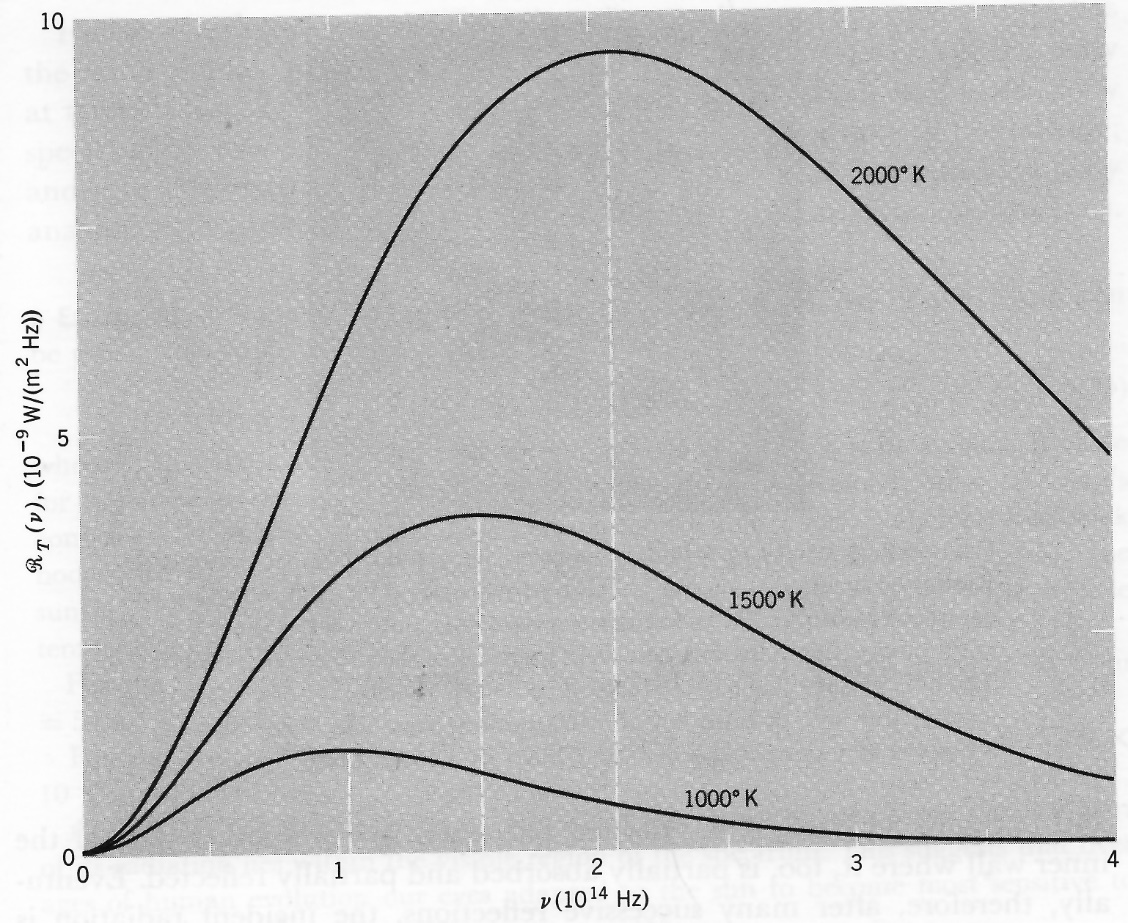
\includegraphics[width=5.125in,height=4.19792in]{images/05_planck/image001.jpg}
  \caption*{\textbf{Figure 1}. \emph{The observed spectral radiancy of a black body
  $\Re_T$, as a function of frequency $\nu$ of
  radiation, shown for black body temperatures of 1000$^\circ$, 1500$^\circ$, and 2000$^\circ$
  Kelvin. The total energy emitted per unit time per unit area (radiancy
  \emph{R\textsubscript{T}}, or area under the curve) increases rapidly
  with temperature. Note that the frequency of maximum spectral radiancy
  (dashed line) increases linearly with temperature (Wien's displacement
  law). The visible region of the spectrum is off scale to the right,
  yellow being at about 5 x 10\textsuperscript{14} Hz. Most of the
  radiation is in the infrared at these temperatures.}}
  \end{center}
\end{figure}
%
of $\Re_T(\nu)$ on $\nu$ and \emph{T}. For a given
value of the frequency $\nu$, we see that the spectral radiancy
$\Re_T(\nu)$ increases with increasing temperature
\emph{T}. If we integrate the quantity $\Re_T(\nu)$ over
all frequencies $\nu$ we obtain the total energy emitted per unit
time per unit area from a black body at temperature \emph{T}. This
quantity
%
\begin{equation}
R_T = \int_{0}^{\infty}\! \Re_T(\nu)\, d\nu
\end{equation}
%
is called the \emph{radiancy}, appropriate units for it being
watts/m$^2$. It can be interpreted as the area under a
curve in Fig. 1, from which we see that it increases rapidly as the
temperature increases. The exact dependence of radiancy on temperature
is given by \emph{Stefan's law},
%
\begin{equation}
R_T = \sigma T^{4},
\end{equation}
%
in which $\sigma = 5.67 \times 10^{-8}$ watt/(m\textsuperscript{2} $^\circ$K\textsuperscript{4}) is a universal
constant called the Stefan-Boltzman constant. We also see from Fig. 1
that as the temperature \emph{T} increases, the spectral distribution of
frequencies shifts to higher values. If the frequency $\nu$ at which
$\Re_T(\nu)$ reaches its maximum value is called
$\nu_{max}$, then as \emph{T} increases
$\nu_{max}$ is displaced toward higher frequencies. This
relation,
%
\begin{equation}\tag{3a}
\nu_{max} \propto T
\end{equation}
%
is called \emph{Wien's displacement law} {[}discovered in 1894{]}. These
experimental results are consistent with the observations we discussed
earlier, namely that the quantity of thermal radiation increases rapidly
with temperature (a hot body radiates much more heat energy at higher
temperatures) and that the principal frequency of the radiation becomes
higher with increasing temperature (the color of a hot body changes from
red to white to blue).

Most black bodies used in laboratory experiments are cavities (ovens)
having a very small opening. Let's explain why such a cavity, shown
schematically in Fig.\ 2, is a black body. Radiation outside the cavity
can enter it through the hole. It then strikes the inner wall, where it
is partially absorbed and partially reflected. The reflected part then
strikes another part of the inner wall where it, too, is partially
absorbed and partially reflected. Eventually, therefore, after many
successive reflections, the incident radiation is totally absorbed by
the wall. Because the area cut out by the hole is such a very small part
of the total area of the cavity wall, we can safely neglect the (very
small) amount of the incoming radiation that can be
%
\begin{figure}[h]
  \begin{center}
  \captionsetup{width=.75\textwidth}
  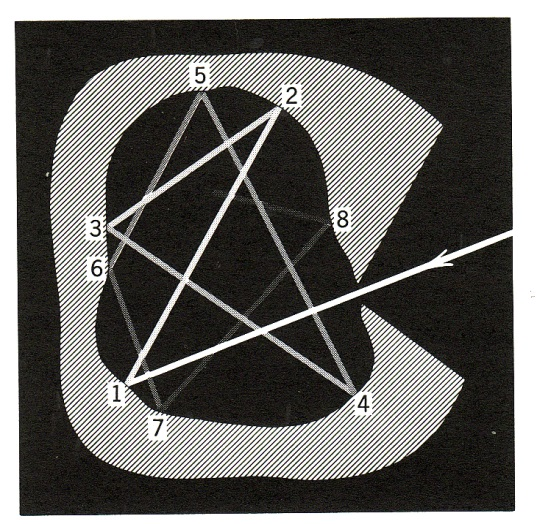
\includegraphics[width=2.4375in,height=2.38542in]{images/05_planck/image007.jpg}
  \caption*{\textbf{Figure 2}. \emph{A cavity in a body connected by a small hole to the
    outside. Radiation incident upon the hole is partly absorbed on each
    reflection and completely absorbed after many successive reflections on
    the inner surface of the cavity. (Note the diminution in intensity of
    the successive reflections.) The hole absorbs like a black body. . . .
    The hole emits like a black body.}}
  \end{center}
\end{figure}
%
reflected back out through the hole. For practical purposes we can say
that all the radiation incident on the hole from the outside is absorbed
by it. Therefore, the hole behaves just as the surface of a black body
behaves, i.e., it absorbs all the radiation incident on it. Indeed, at
low temperatures the hole appears black. If we raise the temperature by
heating the cavity walls uniformly, the hole will become self-luminous.
The inner walls emit thermal radiation into the cavity and some very
small part of this radiation will emerge from the interior through the
hole. Since the hole acts like a black surface, the spectrum of
radiation emitted by it will be characteristic of a black body.

Of course, the thermal radiation emitted by the hole is just a specimen
of the radiation filling the cavity. Therefore, the radiation inside the
cavity also has a spectrum characteristic of a black body. Since the
hole acts as a black surface, the spectrum emitted by the hole in the
cavity whose walls are at a temperature \emph{T} can be described, as
before, by the spectral radiancy $\Re_T(\nu)$. But the
spectrum of radiation \emph{inside} the cavity, called \emph{cavity
radiation}, is more conveniently described by the \emph{energy density}
$\rho_T(\nu)$, which gives the energy in the frequency
interval $\nu$ to $\nu\! +\! d\nu$ per unit volume of the cavity
at temperature \emph{T}. These quantities are proportional to one
another; that is,
%
\setcounter{equation}{3}
\begin{equation}
\rho_T(\nu) = (8\pi/c) \Re_T(\nu) \text{[equation modified]}
\end{equation}
%
. . . Suppose that we uniformly heat to a temperature \emph{T} a piece
of metal containing a cavity. The electrons in the metallic walls are
thermally agitated and emit electromagnetic radiation into the cavity.
Thermal equilibrium is established and maintained in the cavity by the
absorption and re-radiation of energy by the walls.
\end{quotation}

One attempt to understand the phenomenon of black body radiation was
that of Lord Rayleigh and Sir James Jeans. By 1905 their combined
efforts had led to the derivation of a formula for
$\rho_T(\nu)$.

\begin{quotation}
Rayleigh and Jeans showed that the radiation inside such a cavity of
volume \emph{V} consists of standing waves with nodes at the walls. They
computed the number of standing waves in the frequency interval $\nu$
to $\nu + d\nu$ to be
%
\begin{equation}
N(\nu)\, d\nu = \frac{8\pi V}{c^3}\nu^{2}\, d\nu % eqn (5)
\end{equation}
%
in which \emph{c} is the velocity of electromagnetic waves. Now, each
such standing wave contains energy. The average energy per wave, when
the system is in thermal equilibrium, can be determined from the
\textbf{classical} \emph{law of equipartition of energy}.... This states
that the average energy {[}per wave{]} is the same for each standing
wave in the cavity, independent of its frequency, i.e., the energy is
partitioned equally over all frequencies; the value of the average
energy $\bar{\varepsilon}$ depends only on the temperature \emph{T} and is given by
%
\begin{equation}
\bar{\varepsilon}(\nu, T) = \bar{\varepsilon}(T) = kT % eqn (6)
\end{equation}
%
where \emph{k} (= $1.37 \times 10^{-23}$ joule/$^\circ$K) is the
Boltzman constant. To get the average energy content per unit volume of
cavity in the frequency interval $\nu$ to $\nu\! +\! d\nu$, we
simply multiply the number of standing waves in the frequency interval
by the average energy of a wave and divide by the volume of the cavity.
In this way {[}based on the classical law of equipartition{]}, Rayleigh
and Jeans found the energy density $\rho_T(\nu) d\nu$ to be
%
\begin{equation}
\rho_T(\nu) d\nu = \frac{8\pi \nu^2}{c^3}kT\, d\nu, % eqn (7)
\end{equation}
%
which is called \emph{the Rayleigh-Jeans formula for black-body
radiation}.\footnote{Rayleigh realized in 1900 that Equation 7
  contradicted Wien's displacement law (Eq. 3a). In 1911 Paul Ehrenfest
  pointed out that it also implied what was called ``the ultra-violet
  catastrophe.''}

We compare the Rayleigh-Jeans formula, in Fig. 4, with the
experimental result for a cavity radiator at 1500$^\circ$K. As the frequency is
reduced to zero, the spectrum predicted by the Rayleigh-Jeans classical
formula does come closer and closer to the experimentally observed
spectrum. However, as the frequency is increased to large values
(ultraviolet region of the spectrum), the classical theoretical
result diverges enormously from experiment. Indeed, the classical
formula predicts an infinite energy density whereas experiment shows
that the energy density goes to zero at very high frequencies. This
completely erroneous prediction of classical physics was regarded as
such a serious shortcoming that it came to be called ``the ultraviolet
catastrophe.''

%\includegraphics[width=3.67708in,height=2.39583in]{media/image9.jpeg}
%
\begin{figure}[h]
  \begin{center}
  \captionsetup{width=3.67708in}
  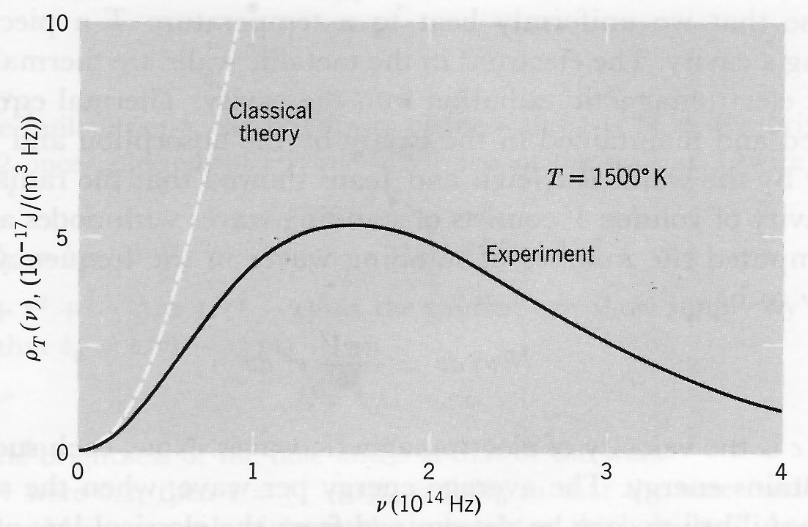
\includegraphics[width=3.67708in,height=2.39583in]{images/05_planck/image017.jpg}
  \caption*{\textbf{Figure 4}. \emph{The Rayleigh-Jeans prediction (dashed line) compared
    with the experimental result (solid line) for the energy density of a
    black body, showing the ultraviolet catastrophe.}}
  \end{center}
\end{figure}
%
\end{quotation}

In 1900 Max Planck made an independent attempt to understand black body
radiation. He began by letting $\bar{\varepsilon}(\nu, T)$ stand for the average
energy of an electromagnetic wave of frequency $\nu$ at temperature
\emph{T}, and then was able to demonstrate theoretically that when the
walls and the radiation within the cavity are in equilibrium, the energy
density, $\rho_T(\nu)$, is related to the average
energy per wave at $\nu$ and \emph{T}, $\bar{\varepsilon}(\nu, T)$, as follows:
%
\setcounter{equation}{9}
\begin{equation}
\rho_T(\nu)\, d\nu = \frac{8\pi \nu^2}{c^3}\bar{\varepsilon}(\nu, T)\, d\nu. % eqn (10)
\end{equation}
%
In an effort to arrive at an expression for $\rho_T(\nu)$
which would not predict an ultraviolet catastrophe, Planck sought to
determine a formula for $\bar{\varepsilon}$ by trying to fit the graphs of experimental
results. He arrived at the following empirical formula:
\begin{equation}\label{e_eq}
\bar{\varepsilon}(\nu) = \frac{h\nu}{e^{h\nu/kT}-1} \; , % eqn (11)
\end{equation}
where $h$ is a constant.\footnote{The constant $e$ in eq.\! \ref{e_eq} is the number $2.718\dots$ providing the base of natural logarithms. This is different from the "e" in the unit "eV" in the next sentence, an abbreviation for electronvolts.} In particular, it turned out that the
value of this constant $h$ that would give the best fit between his
formula and the experimental data was: $h = 6.63\! \times\!
10^{-34}$ joule-sec $= 4.14\! \times\! 10^{-15}$
eV-sec, which is very nearly the same as the modern value for what has
come to be known as \emph{Planck's constant.}

In Figure 5 we compare Equation 11 with Equation 6, the classical law of
equipartition:
%
\begin{equation*}\tag{6}
\bar{\varepsilon}(\nu, T) = \bar{\varepsilon}(T) = kT % eqn (6 redux)
\end{equation*}
%
%
\begin{figure}[h]
  \begin{center}
  \captionsetup{width=4.15625in}
  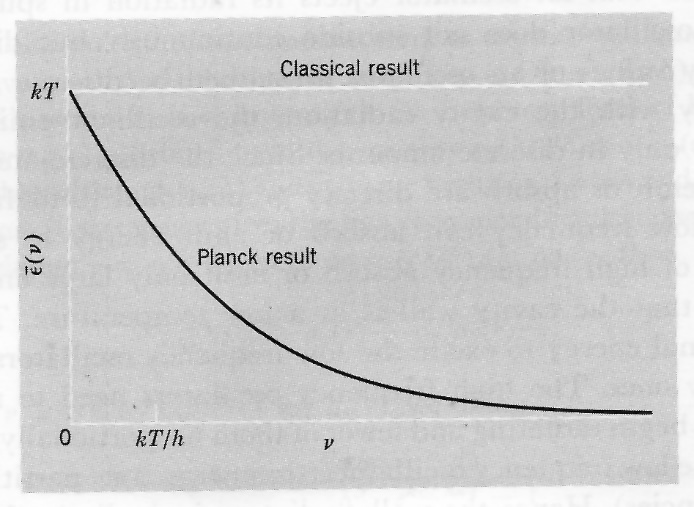
\includegraphics[width=3.15625in,height=2.30208in]{images/05_planck/image028.jpg}
  \caption*{\textbf{Figure 5}. \emph{Planck's formula for the average value of the energy,
    as a function of frequency, compared with the classical result.}}
  \end{center}
\end{figure}
%
\begin{quotation}
{[}N{]}ote that $\nu$ drops from \emph{kT} to zero in a continuous
way with increasing frequency, at first rapidly and then slowly.

When Planck used his result (Eq. 11) for $\bar{\varepsilon}$ rather than the classical value
$\bar{\varepsilon} = kT$ (Eq. 6) in the calculation of the energy density in the
cavity radiation spectrum, he found
\begin{equation}
\rho_T(\nu)\, d\nu = \frac{8\pi\nu^2}{c^3} \frac{h\nu}{e^{h\nu/kT}-1} d\nu \; . % eqn (12)
\end{equation}
This is \emph{the Planck formula for black body radiation}. Figure 6
shows a comparison of this result of Planck's {[}calculations{]} with
experiment for a temperature \emph{T} = 1595$^\circ$K. The experimental results
are in complete agreement with Planck's formula at all temperatures.

%\includegraphics[width=3.6875in,height=2.92708in]{media/image22.jpeg}
%
\begin{figure}[h]
  \begin{center}
  \captionsetup{width=4.6875in}
  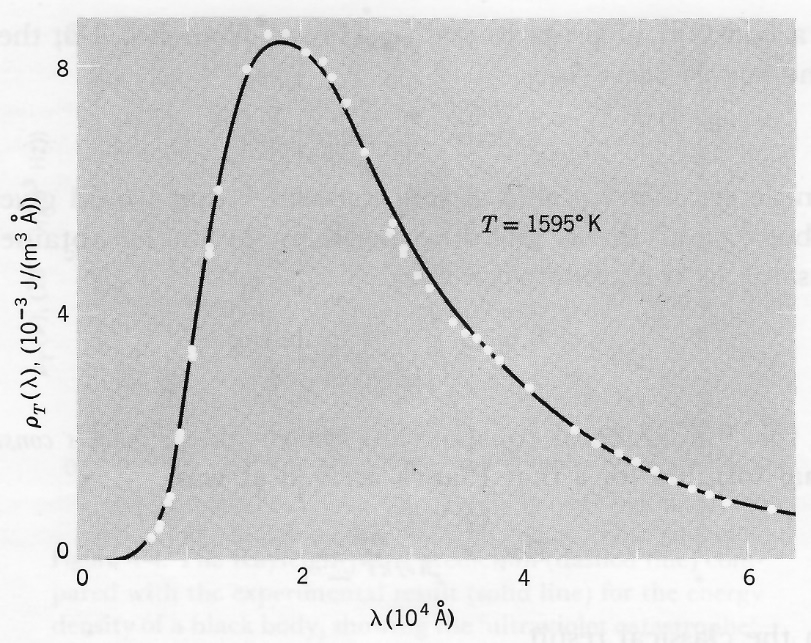
\includegraphics[width=3.6875in,height=2.92708in]{images/05_planck/image037.jpg}
  \caption*{\textbf{Figure 6}. \emph{Planck's energy density prediction (solid line)
    compared to the experimental results (circles) of the energy density of
    a black body. The data were reported by Coblentz in 1916 and apply to a
    temperature of 1595$^\circ$K. The author remarked in his paper that after
    drawing the spectral energy curves resulting from his measurements,
    ``owing to eye fatigue, it was impossible for months thereafter to give
    attention to the reduction of the data.'' The data, when finally
    reduced, led to a value of Planck's constant of 6.57 x
    10\textsuperscript{-34} J-sec.}}
  \end{center}
\end{figure}
\end{quotation}

\vspace{5pt}

\section*{B. Black Body Radiation: Planck's \emph{Theoretical}
Determination of the Formula That Fit the Experimental Results.}

Up to this point Equation 12 is merely an \emph{ad hoc} formula based on
Equation 11, which had been constructed to fit the experimental results.
Planck was convinced that it was right. Yet, theorist that he was, he
wanted more: he wanted a \emph{theoretical} derivation of Equation 11
that would explain why it was so, giving it physical meaning. We shall
ignore most of the details and, instead, focus on Planck's fundamental
modification of the classical view.

In thinking about the black-body problem, Planck had been guided by
Hertz's discovery (which may have been demonstrated in Junior
Laboratory) that oscillating charged particles---parts of tiny elastic
systems of some sort---presumably parts of atoms---emit electromagnetic
waves, which meant that cavity radiation must originate in
submicroscopic electric oscillators in the cavity walls. He reasoned
that heating a material body ought to set microscopic systems of charged
particles vibrating, for according to Maxwell they should be made to
resonate harmonically by incoming light of the proper frequencies, and
they would also be jostled by the vibratory heat motions of their
neighbors. In turn a vibrating electric charge should generate light of
the same frequency as its own vibration, again in accordance with
Maxwell's theory.

Furthermore, since the character of cavity radiation had been shown to
be independent of the material of the cavity walls, Planck had felt free
to make possibly artificial assumptions about the character of the
oscillators: He had supposed them all to be \emph{simple harmonic
oscillators}. In this analogy, Planck imagined that the cavity walls
consisted of tiny `springs' of force constants $\beta$, on the ends of
which were charged particles of masses \emph{m}. As we saw in Junior
Laboratory, this meant that each such oscillator would have a natural
frequency given by
\begin{equation}
\nu = \frac{1}{2\pi}\sqrt{\frac{\beta}{m}} \; . % eqn (13)
\end{equation}
That is, each of them had its own fixed frequency, determined by the
force binding the charge to its equilibrium position, and by the mass of
the charge.

Since the range of frequencies in cavity radiation is assumed to be
continuous, the assumption must be that the cavity walls contain large
numbers of oscillators of all frequencies represented in the radiation.
When any oscillator is vibrating at its fixed frequency, it is radiating
electromagnetic waves of the same frequency; and it is losing energy.
The temperature of the cavity walls will drop unless the lost energy is
replaced. It can be replaced by absorption of radiant energy; each
oscillator will absorb energy only of its natural frequency. But the
energy can also be replaced by heat supplied to the cavity walls: The
cavity is kept in a constant-temperature oven. The available energy will
be constantly re-distributed among the various oscillators, because of
their constant absorption and radiation of energy.

Considering the temperature \emph{T} to be fixed, Planck set out to
determine how, on the average, the total amount of energy in the cavity
at temperature \emph{T} would distribute itself on the average among the
various oscillators of different natural frequencies, $\nu$, of
vibration. That is, Planck tried to \emph{derive} the formula for
$\bar{\varepsilon}(\nu)$ (Eq. 11), which he had already arrived at by matching the
experimental results. This \emph{equilibrium distribution} of energy
among the oscillators will, in turn, determine how the energy density,
$\rho_T(\nu)$, of the cavity radiation varies with
frequency.

So, Planck had to answer the question: If, of the portions of energy
given to all the oscillators at a given moment, we consider the subset
consisting of those amounts of energy allotted to the oscillators of
natural frequency $\nu$, how do those amounts of energy distribute
themselves among the latter? Planck's first insight was that his
question was analogous to a question that had already been answered by
Ludwig Boltzmann, namely: How does the energy allotted to a set of gas
molecules in a closed container at a constant temperature \emph{T}
distribute itself among the individual molecules? These molecules have
an average kinetic energy, which is the analogue to Planck's $\bar{\varepsilon}(\nu)$.
Stated as a proportion the analogy is roughly:

\begin{quote}
(all gas molecules in the container) : (all oscillators of natural
frequency $\nu$ in the cavity walls) :: (all gas molecules in the
container having energy $\varepsilon$) : (all oscillators of natural
frequency $\nu$ having energy $\varepsilon$ in the cavity walls).
\end{quote}

Because of the large numbers of molecules and because of the fact that
they are constantly colliding, Boltzmann assumed that the energy
eventually became distributed among the molecules in a stable way. Using
probability theory as well as mechanics, Boltzmann imagined that, at any
given time, each of the $N$ molecules in a given volume of a gas would
have one of, say, $n$ different energy states. His problem was to
find the probability of the various possible distributions of particles
among these $n$ energy states. By calculating the total number of
ways in which each such distribution could be achieved, Boltzmann was
able to determine the most probable distribution of particles among the
available energy states. That is, for each of the available energy
states, $\varepsilon$, he determined the fraction,
$\Delta N_{\varepsilon}/N$, of the total number of molecules,
\emph{N,} that had energy $\varepsilon$, in the most probable distribution:
%
\begin{equation}
\frac{\Delta N_{\varepsilon}}{N} \propto e^{-{\varepsilon}/kT} % eqn (14)
\end{equation}
%
where \emph{e} is the base of natural logarithms, \emph{T} is the
absolute temperature, and \emph{k} is Boltzmann's constant, given by the
gas constant \emph{R} divided by Avogadro's number. The proportionality
(14) implies that the fraction $\Delta N_{\varepsilon}/N$
decreases as $\varepsilon$, the energy state considered, increases.

In order to find the way energy would distribute itself among his
hypothetical oscillators, Planck made use of the Boltzmann distribution
(14). He proceeded in somewhat the following way.

Consider an oscillator of mass $m$ and force constant $\beta$; let
its displacement be $x$ and its momentum $p$ =
$m(dx/dt)$. Its potential energy will be
$(1/2)\beta x^2$ and its kinetic energy $(1/2)m(dx/dt)^{2} = p^{2}/2m$.
Therefore, its total energy is\footnote{You may want to review the
  second semester junior lab manual treatment of the pendulum for what
  follows. Potential energy should equal the work done against the
  restoring force in moving the mass $m$ from zero to displacement
  $x$. The restoring force is $F = - \beta x$. Therefore the
  potential energy is this force integrated from 0 to $x$. One must
  integrate over $x$ rather than write $Fx$ because the force
  varies with $x$.}

\begin{equation}
\varepsilon = \frac{p^2}{2m} + \frac{\beta x^2}{2} % eqn (15)
\end{equation}

Its frequency, which should be regarded as fixed in what follows, is
given by Equation 13.

Equation 15 can be viewed as the equation of an ellipse in the
(\emph{p,x}) plane (this plane is called the \emph{state domain} by
Planck), where $\sqrt{2m\varepsilon}$ and $\sqrt{2\varepsilon/\beta}$ are the semi-minor and
semi-major axes\footnote{According to the Sophomore Mathematics manual,
  \emph{A Cartesian Survey of the Conic Sections}, when the equation for
  an ellipse centered at the origin is put into standard form:\\
  \(\frac{x^{2}}{a^{2}} + \frac{y^{2}}{b^{2}} - 1 = 0\), according as
  $a$ is greater or less than $b$, the major axis is of
  length $2a$, along the $x$-axis, or of length $2b$,
  along the $y$-axis.} of the inmost ellipse in Figure 7, labeled
  $\varepsilon = h\nu$. The area of the inmost ellipse will be\footnote{Given
  the equation of the ellipse in the previous note, one-fourth of the
  ellipse would correspond to $y = b[1 - (x/a)^2]^{1/2}, x \geq 0$.

  Then the area contained by the ellipse would be given by:

  \({A = \ 4\int_{0}^{a}{b(1 - \frac{x^{2}}{a^{2}}})}^{1/2}dx = \ \frac{4b}{a}\int_{0}^{a}{({a^{2} - \ x^{2})}^{\frac{1}{2}\ }}dx = \ \frac{4b}{a}\lbrack\frac{x}{2}({a^{2} - \ x^{2})}^{\frac{1}{2}\ } + \ \frac{a^{2}}{2}\sin^{- 1}({\frac{x}{a})}\rbrack_{0\ }^{a} = \ \pi ab\),

  where the indefinite integral is found from a table of integrals.}
%
\begin{equation}
A_1 = \pi p_{max}x_{max} = \pi\sqrt{2m\varepsilon}\sqrt{2\frac{\varepsilon}{\beta}} = 2\pi\varepsilon\sqrt{m/\beta} = \frac{\varepsilon}{\nu}. % eqn (16)
\end{equation}
%\includegraphics[width=4.13542in,height=2.38542in]{media/image29.png}
%
\begin{figure}[h]
  \begin{center}
  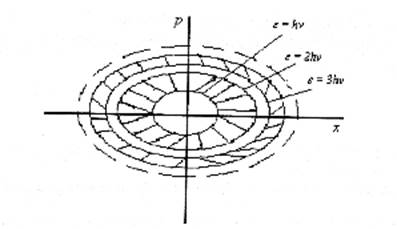
\includegraphics[width=4.13542in,height=2.38542in]{images/05_planck/image050.jpg}
  \caption*{\textbf{Figure 7}. \emph{Ellipses in the state domain.}}
  \end{center}
\end{figure}
%
Let us define a constant $h$, such that $h = A_1 = \varepsilon/\nu$. Previously Planck had showed that the area integral,
$\int\! dp\, dx$, does not vary over time. One way to think of this is to
notice that if each of the points $(p,x)$ inside the inmost ellipse
is given an additional energy of $h\nu$ (for example, by pushing a
pendulum or a spring with an additional force), then each of these
points will be displaced to the annular region between the ellipses
labeled $\varepsilon = h\nu$ and $\varepsilon = 2h\nu$, respectively (the inmost
cross-hatched annulus in the diagram). Thus, this annular region, equal
to the area of the second ellipse, $A_2$, minus that
of the first, $A_2 - A_1$,
also has area $h$, as does every annular region between two
consecutive ellipses. The entire state domain (the
${[}\emph{p,x}{]}$-plane) is thus naturally divided into non-overlapping
areas of size $h$, each of which corresponds to an amount of energy
= $h\nu$. It remains to associate a probability with each annular
region and then to take the limit of the sum of these probabilities as
the areas of the annular regions shrink to zero. But this is given to us
by the Boltzmann distribution, Equation 14.

Identifying $\varepsilon$ in Equation 14 with $h\nu$ gives us the result
that the probability of an oscillator of frequency $\nu$ having
energy $\varepsilon = h\nu$, that is, $P(\nu, h\nu)$, or, equivalently, the
fraction of the total number of oscillators of frequency $\nu$ that
have energy $\varepsilon = h\nu$, $\Delta N_\varepsilon/N$,
is
%
\begin{equation*}
P(\nu, h\nu) = Ce^{-h\nu/kT}.
\end{equation*}
%
(\emph{C} is the constant of proportionality, to be determined.)
Analogously, for any whole number \emph{n}, we obtain that the
probability of an oscillator of frequency $\nu$ having energy
$n\varepsilon = nh\nu$ is

\begin{equation}
P(\nu, nh\nu) = Ce^{-nh\nu/kT}. % eqn (17)
\end{equation}

This is the probability associated with the annular region between the
ellipses $\varepsilon = (n-1)h\nu$ and $\varepsilon = nh\nu$.

The constant \emph{C} is determined by adding up all the probabilities, 
which must equal 1;\footnote{The last step to the equation relies on an
  identity that is part of the "toolkit" of physicists and
  mathematicians, derivable using Taylor's theorem:

  \emph{(1 - x)\textsuperscript{-1} = 1 + x + x\textsuperscript{2} +
  x\textsuperscript{3} + \ldots{}}

  We let $x = e^{-h\nu/kT}$, and writing out
  some of the summation, we find that the identity is applicable.}
%
\begin{equation}
\sum_{n=0}^{\infty} P(\nu, nh\nu) = \sum_{n=0}^{\infty} Ce^{-nh\nu/kT} = C(1 - e^{-h\nu/kT})^{-1} = 1, % eqn (18)
\end{equation}
%
from which it follows that
\begin{equation}
C = 1 - e^{-h\nu/kT}. % eqn (19)
\end{equation}
If we want to find the average energy, $\bar{\varepsilon}(\nu, T)$, of \emph{all} the
oscillators having the frequency $\nu$ at temperature \emph{T}, we
multiply each of the energies, $h\nu$, $2h\nu$, $3h\nu$, \ldots
, by the probability of an oscillator's having that energy, and add up
all the terms:
%
\begin{equation}
\bar{\varepsilon}(\nu, T) \approx Ch\nu\left(e^{-h\nu/KT}+2e^{-2h\nu/kT}+\cdots\right) = Ch\nu e^{-h\nu/kT}\left(1-e^{-h\nu/kT}\right)^{-2}. % eqn (20)
\end{equation}
%
where, be it noted, we have had to include the possibility that an
oscillator have zero energy.\footnote{We have again made use of an
  identity, derivable from Taylor's Theorem,

  \emph{(1 -- x)\textsuperscript{-2} = 1 + 2x + 3x\textsuperscript{2} +
  4x\textsuperscript{3} + \ldots{} }

  And we again let $x = e^{-h\nu/kT}$ and
  factor that out, then use this identity to get the last expression in
  Equation 20.} Substituting our value for \emph{C}, (19), into Equation
20, we obtain for the average energy of the oscillators of frequency
$\nu$ at temperature \emph{T:}\footnote{The equation gets its
  right-hand form by multiplication of both numerator and denominator by
  $e^{h\nu/kT}$.}
%
\begin{equation}
\bar{\varepsilon}(\nu, T) \approx \frac{h\nu e^{-h\nu/kT}}{1-e^{-h\nu/kT}} = \frac{h\nu}{e^{h\nu/kT}-1}, % eqn (21)
\end{equation}
%
which would be identical with Equation 11 if the ``$\approx$'' were replaced
by ``=.``

We observe that, so far, Planck has been considering finite increments
in energy, of amount $h\nu$. Equation 21 is thus, according to the
notions of all earlier physics, only approximate; to obtain the exact
expression, it would normally be necessary to take the limit of Equation
21 as \emph{h} goes to zero. If this is done, however, we find
that\footnote{We let $a = h\nu/kT$, and we also recall that from
  junior math, $e^a$ is expressible in the form
\begin{equation*}
e^a = 1 + a + \frac{a^2}{2!} + \frac{a^3}{3!} + \cdots + \frac{a^n}{n!} + \cdots
\end{equation*}
  If we now write
\begin{equation*}
\bar{\varepsilon}(\nu, T) = \frac{kTa}{e^a - 1}
\end{equation*}
  and expand \emph{e\textsuperscript{a}}, the denominator will go to
  \emph{a} as \emph{h} and \emph{a} go to zero, which cancels with the
  \emph{a} in the numerator, leaving \emph{kT}.}
%
\begin{equation*}
\bar{\varepsilon}(\nu, T) \rightarrow kT\quad \text{as}\quad h \rightarrow 0.
\end{equation*}
%
Substituting this expression---$\bar{\varepsilon}(\nu, T) = kT$ {[}Eq.
6{]}---for the average energy into Equation 10, gives for the energy
density the Rayleigh-Jeans formula, Equation 7, which, as we have seen,
is in disagreement with experiment and is theoretically unacceptable in
that it implies the ``ultraviolet catastrophe.''

Now, in the classical calculation of the average energy of a large
number of things of the same kind in thermal equilibrium with each other
at temperature \emph{T} (a calculation that leads to the Equipartition
Law, Eq.\ 6), it was assumed that the energy $\varepsilon$ was a continuous
variable. However, as we have seen, Equation 21, \emph{without taking
the limit}, implies an equation for the energy density, Equation 12,
that accords with experiment (Fig.\ 6). Thus, in order to derive the
equation which fits the experimental results, Planck was forced to say
that the correct expression for $\bar{\varepsilon}(\nu, T)$ must be, not the
approximate Equation 21, or the exact equation resulting from allowing
the annular regions to shrink, but rather Equation 11. In other words,
he had to deny the assumption that the energy $\varepsilon$ varies
continuously. He could not allow \emph{h} to approach zero but, instead,
had to assume that the amount of energy assigned to an oscillator of
frequency $\nu$ must be an integral number of units $\Delta\varepsilon = h\nu$ of
energy---``energy \emph{quanta},'' as Planck called them---where
\emph{h} was the non-zero constant whose value he had determined by
fitting his Equation 11 to the empirical data. We have then, for nonzero
\emph{h}, a theoretical formula which describes the empirical results.
What does it mean? How is the meaning of \emph{h} different now as
compared with its meaning when it was first encountered above where it
was defined as $\varepsilon/\nu$?

\begin{quote}
One can understand the results of Planck's assumption physically in this
way. The electromagnetic waves in the cavity originate from radiation
given off by electrons that are thermally agitated and oscillate in the
walls of the cavity. The electronic oscillators in the cavity wall are
pictured classically as radiating their energy smoothly as their motion
gradually subsides. Planck assumed instead that an oscillator ejects its
radiation in spurts. Thus the energy of an oscillator does not subside
continuously but discretely. The allowed energy values of an oscillator
must then be discrete and, as it exchanges energy with the cavity
radiation, the oscillator emits or absorbs radiant energy only in
discrete amounts. Since the discrete energies that an oscillator can
emit or absorb [$\Delta\varepsilon = h\nu$] are directly proportional to its
frequency, the oscillators of low frequency can absorb or emit energy in
small packets whereas those of high frequency absorb or emit only large
energy packets. Now imagine that the cavity wall is at a low
temperature. Then there is sufficient thermal energy to excite the low
frequency oscillators, but not the high frequency ones. The high
frequency oscillators need to receive much more energy to begin
radiating and fewer of them proportionally are activated compared to the
low frequency oscillators (the energy is not partitioned equally over
all frequencies). Hence the walls radiate principally in the long
wavelength region and hardly at all in the ultraviolet. As the
temperature of the wall is raised there is sufficient thermal energy to
activate a larger number of high frequency oscillators and the resulting
radiation shifts its character toward higher frequencies, i.e., toward
the ultraviolet. Hence the Planck assumptions quite naturally lead to
the experimental observations discussed earlier and avoid the
ultraviolet catastrophe of the classical analysis.
\end{quote}

Physicists acknowledged the remarkable predictive power of Planck's
model. Still, the fact that it relied on the quantum hypothesis was
disturbing. It seemed extremely unlikely that actual microscopic
oscillators should only absorb and emit energy in units. Certainly
macroscopic oscillators do not seen to act this way: We can (we believe)
get a pendulum to absorb energy in any continuously varying amount, just
by nudging it right; and an oscillating pendulum seems to give up its
energy to its surroundings continuously. Quantization seemed just as
unlikely to happen in any plausible microscopic picture of the
interactions between atoms and electromagnetic waves in a continuous
medium. Thus, as long as the necessity for the quantum hypothesis was
not overcome, black-body radiation seemed to stand as a question mark to
Maxwell's theory itself.
